\section{Постановка задачи}

\begin{frame}[t]{Проблематика}
    \begin{block}{Проблема}
        Исследование пещер
    \end{block}
    \begin{columns}[T,onlytextwidth]
        \begin{column}{0.59\textwidth}
            Обзор, кто смотрел эту проблему
        \end{column}
        \begin{column}{0.39\textwidth}
            \begin{figure}[H]
                \centering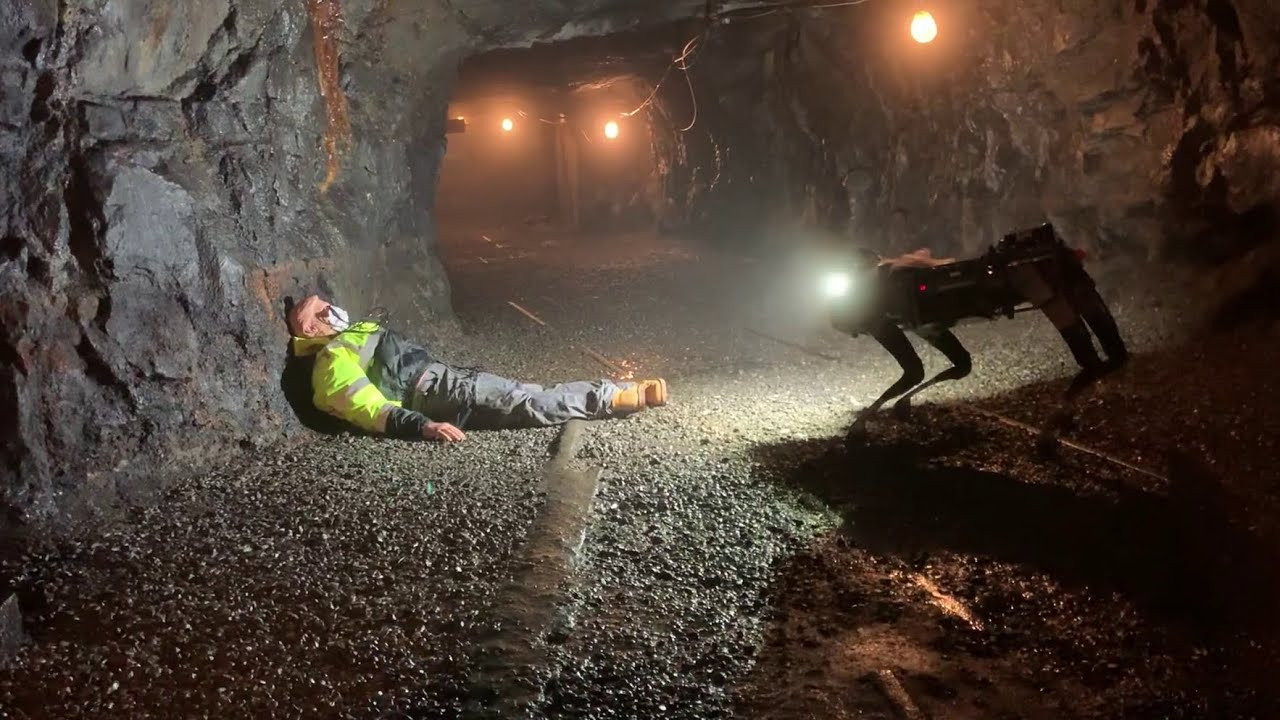
\includegraphics[height=3cm,width=1\textwidth,keepaspectratio]{open_cave.jpg}
                \caption*{DARPA Subterranean Challenge}
            \end{figure}
        \end{column}
    \end{columns}
\end{frame}

\begin{frame}[t]{Предментая область: Пещеры}
    \framesubtitle{}
    \vspace{-0.8cm}
    \begin{figure}[H]
        \begin{subfigure}{0.49\textwidth}
            \begin{subfigure}[b]{0.49\textwidth}
                \centering\includegraphics[height=2.5cm,width=1\textwidth,keepaspectratio,page=1]{./tikz_pictures.pdf}
                \caption{Лужа}
            \end{subfigure}
            \hfill
            \begin{subfigure}[b]{0.49\textwidth}
                \centering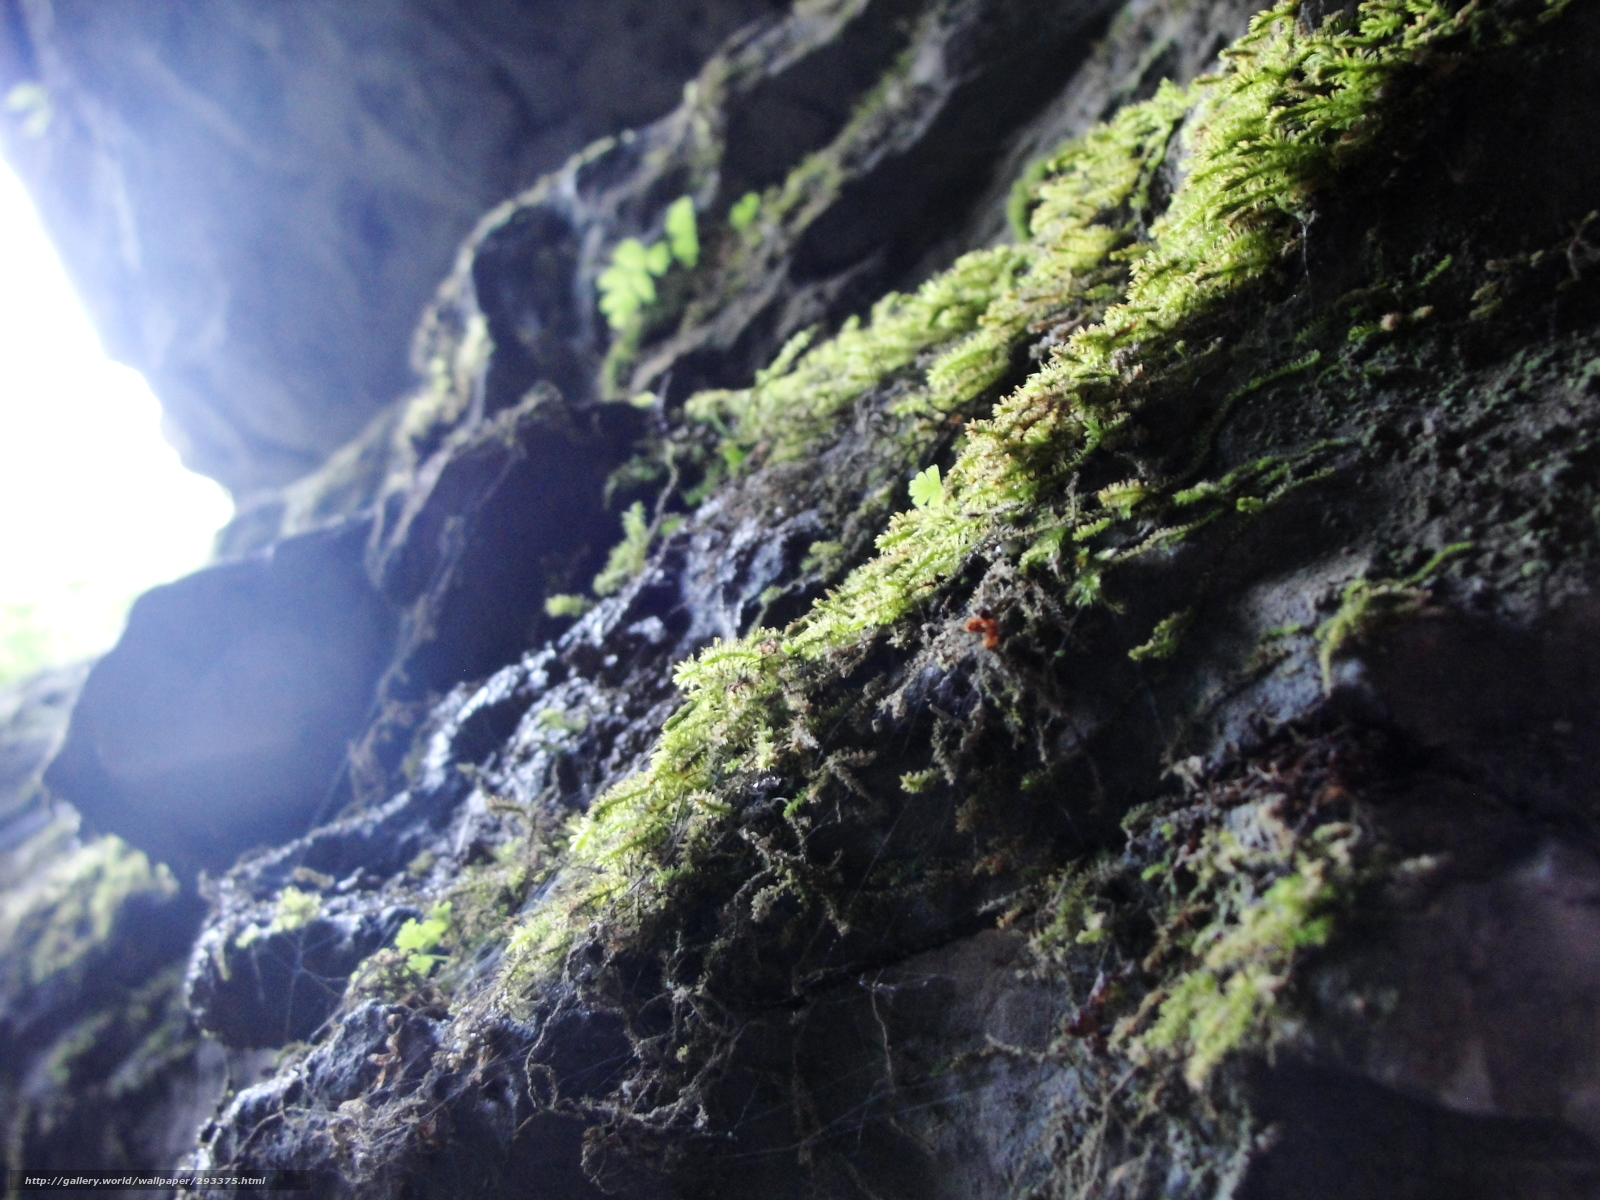
\includegraphics[height=2.5cm,width=1\textwidth,keepaspectratio]{surface_types/moss.jpg}\\
                \caption{Мох}
            \end{subfigure}

            \begin{subfigure}[b]{0.49\textwidth}
                \centering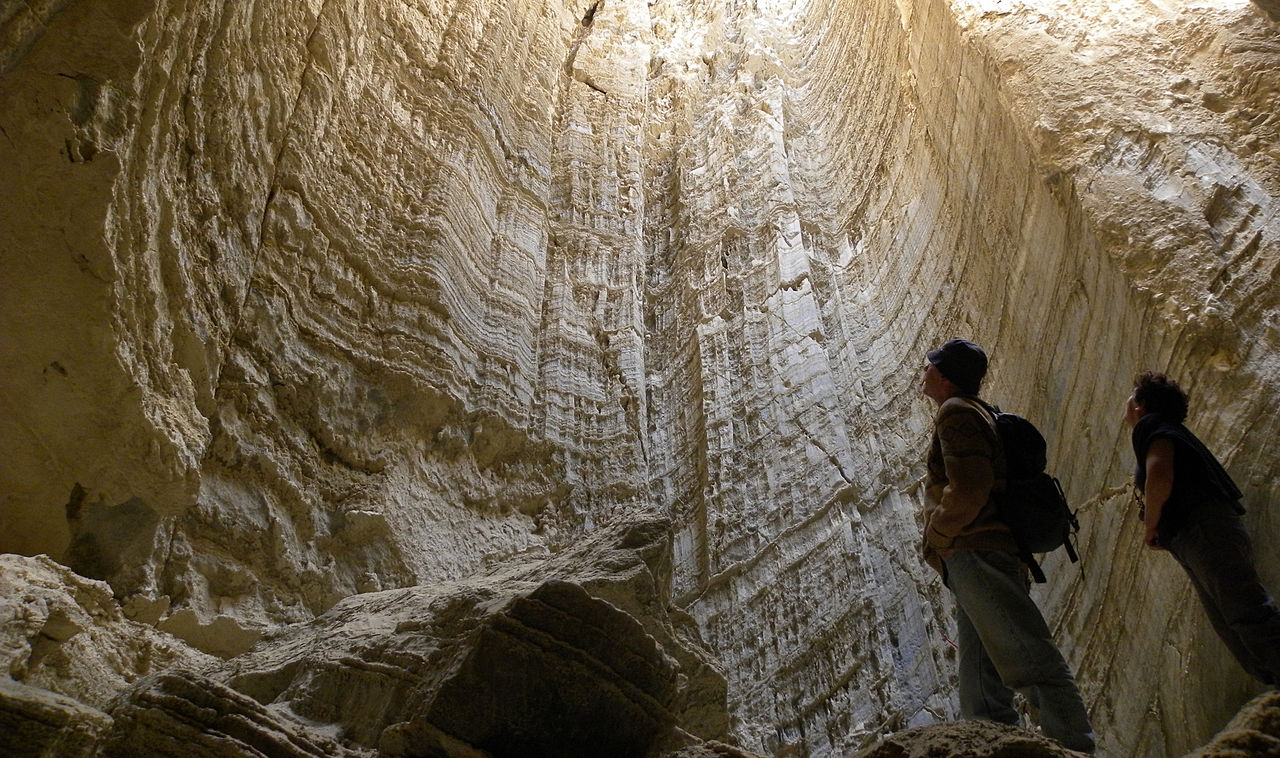
\includegraphics[height=2.5cm,width=1\textwidth,keepaspectratio]{surface_types/salt.jpg}\\
                \caption{Твердые породы}
            \end{subfigure}
            \begin{subfigure}[b]{0.49\textwidth}
                \centering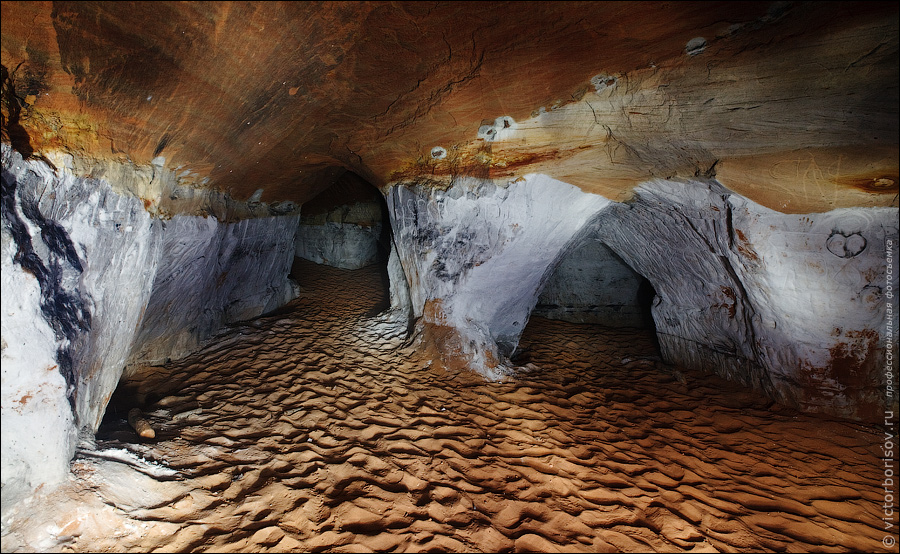
\includegraphics[height=2.5cm,width=1\textwidth,keepaspectratio]{surface_types/sand.jpg}\\
                \caption{Земля}
            \end{subfigure}
            \caption*{Типы опорных поверхностей}
        \end{subfigure}
        \begin{subfigure}{0.49\textwidth}
            \begin{subfigure}{0.99\textwidth}
                \centering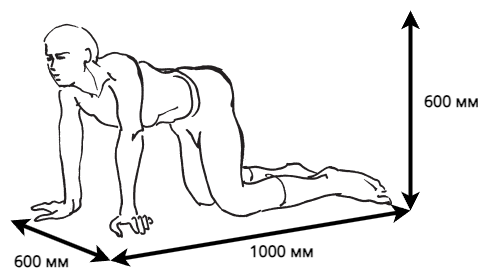
\includegraphics[height=3cm,width=1\textwidth,keepaspectratio]{../images/human_crawling.png}
                \caption*{Габариты пещеры}
            \end{subfigure}

            \begin{subfigure}{0.99\textwidth}
                \centering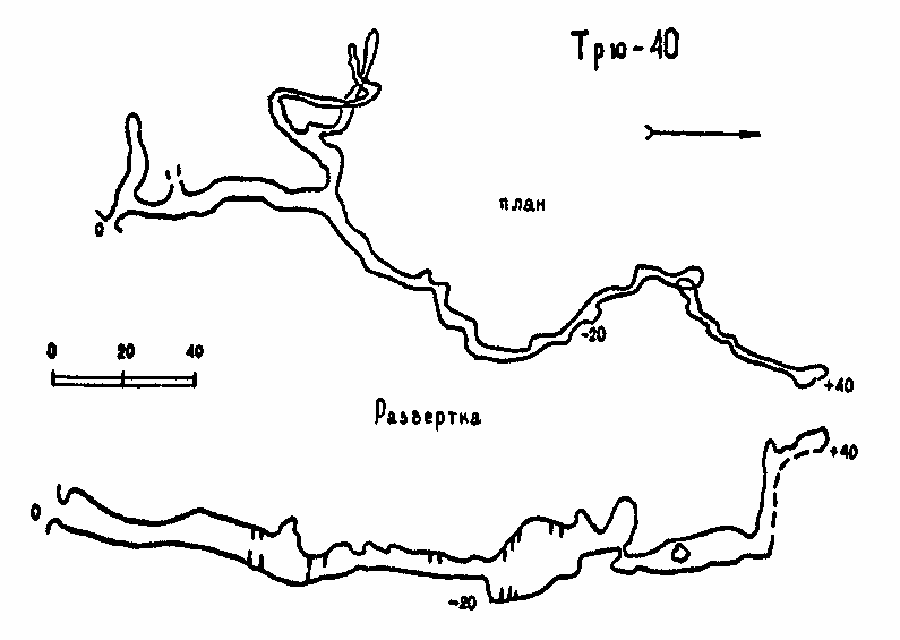
\includegraphics[height=3cm,width=1\textwidth,keepaspectratio]{../images/cave_maps/map3.png}
                \caption*{Протяженность пещер: 1--2 км}
            \end{subfigure}
        \end{subfigure}
    \end{figure}
\end{frame}



\begin{frame}[t]{Вопрос: Как картографировать поверхность под лужей?}
    \framesubtitle{}
    \vspace{-1cm}
    \begin{columns}[T,onlytextwidth]
        \begin{column}{0.44\textwidth}
        \end{column}
        \begin{column}{0.44\textwidth}
            \begin{figure}[H]
                \begin{subfigure}[b]{0.9\textwidth}
                    \centering
                    \centering\includegraphics[height=3.5cm,width=1\textwidth,keepaspectratio,page=2]{./tikz_pictures.pdf}
                \end{subfigure}

                \begin{subfigure}{0.8\textwidth}
                    \centering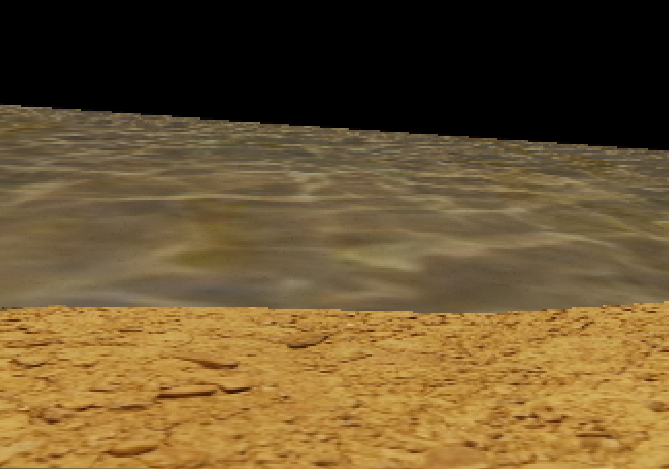
\includegraphics[height=2cm,width=1\textwidth,keepaspectratio]{terrain_w_water_camera.png}
                    \caption*{Вид с камеры}
                \end{subfigure}
            \end{figure}
        \end{column}
    \end{columns}
\end{frame}

\begin{frame}[t]{Цель работы}
    \framesubtitle{}
    Разработать \textbf{метод построения карты местности} с определением \underline{геометрических} и \underline{физико-механических} свойств \textit{опорной поверхности} роботом с шагающими движителями снабженными \underline{тактильными датчиками}, \textit{без использования оптических сенсоров}.
    \begin{figure}[H]
        \begin{subfigure}{0.49\textwidth}
            \centering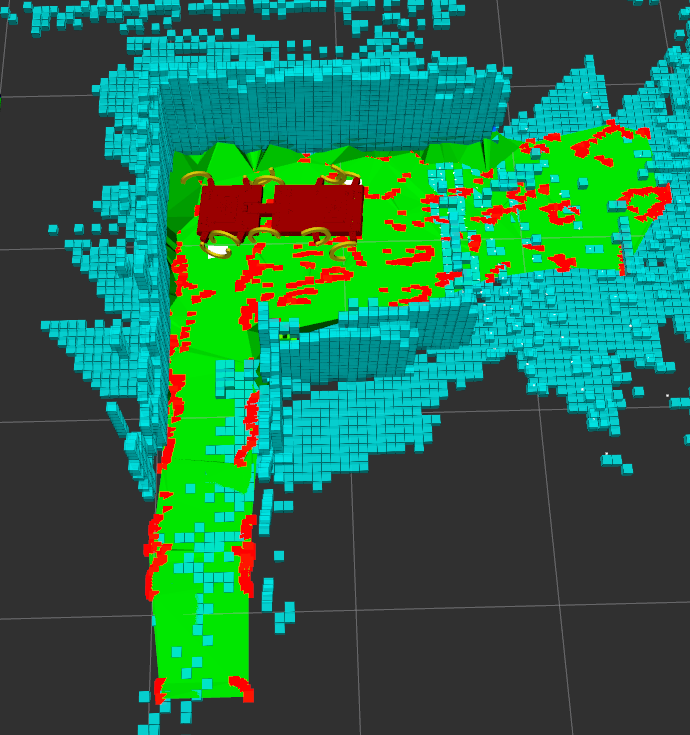
\includegraphics[height=3.5cm,width=1\textwidth,keepaspectratio]{conv_concave.png}
            \caption*{Определение геометрических свойств}
        \end{subfigure}
        \begin{subfigure}{0.49\textwidth}
            \centering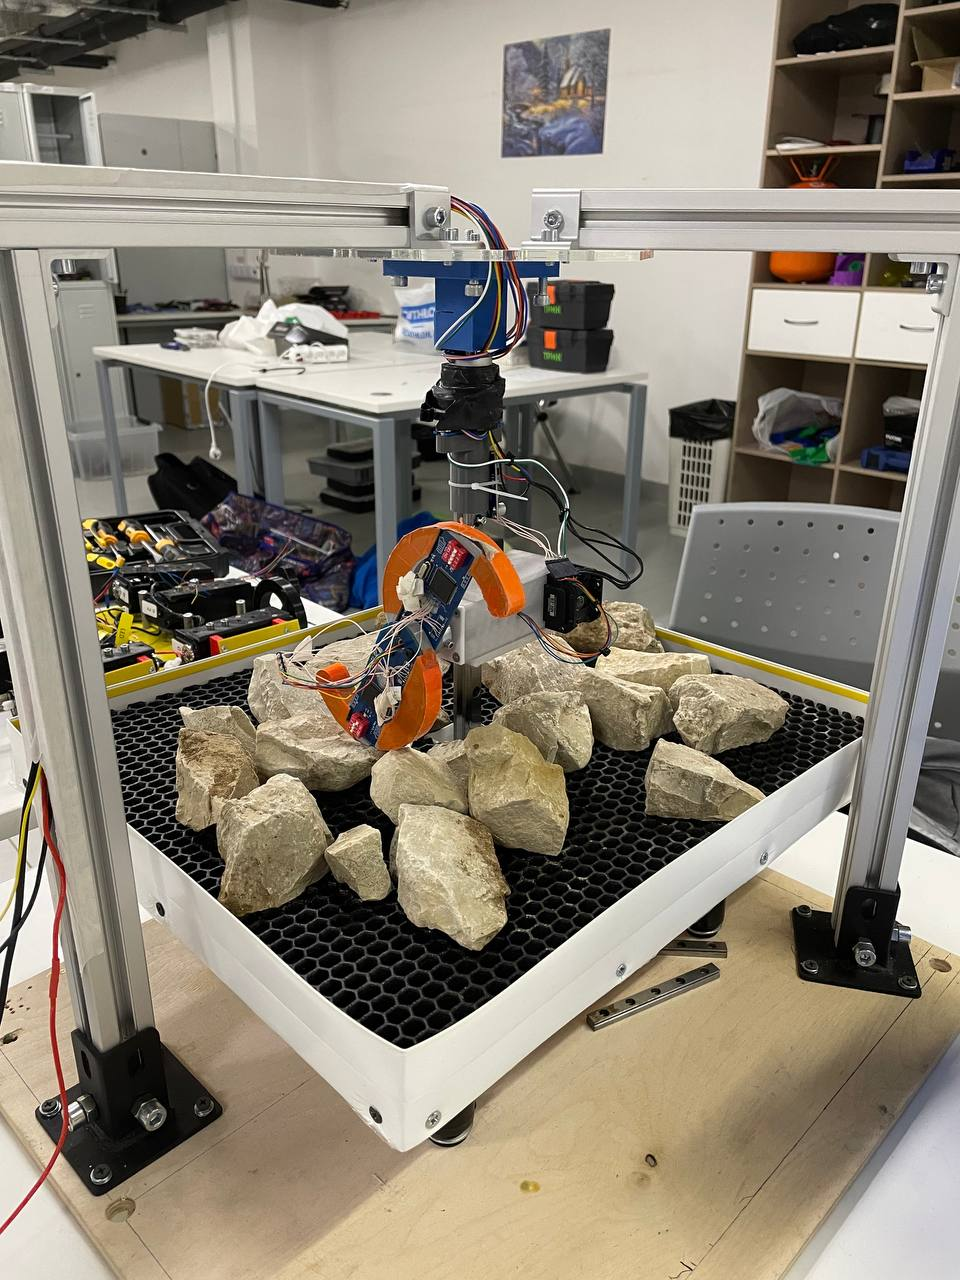
\includegraphics[height=3.5cm,width=1\textwidth,keepaspectratio]{s_shape_leg/view.jpg}
            \caption*{Определение физических свойств}
        \end{subfigure}
    \end{figure}
\end{frame}

\begin{frame}[t]{"1, 2" Построение рельефа местности}
    \framesubtitle{}
    \begin{columns}[T,onlytextwidth]
        \begin{column}{0.49\textwidth}
            \textbf{Геометрические свойства:}\\
            \textit{Входные данные}: следовая дорожка, представленная в виде облака точек.

            \textit{Выходные данные}: полигональная сетка и плотное облако точек.

            \textit{Допустимая точность}: 0.1 м
            \begin{figure}[H]
                \begin{subfigure}[t]{0.49\textwidth}
                    \centering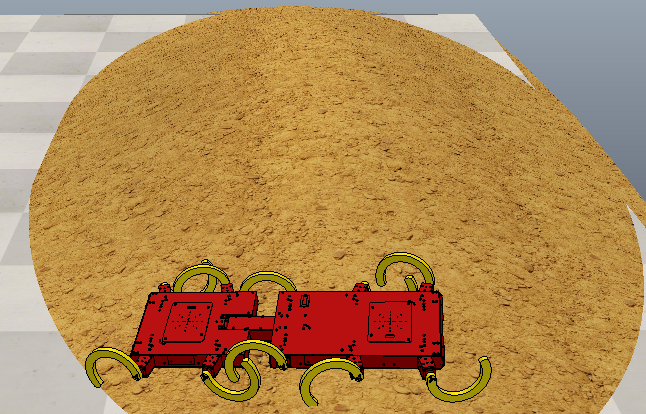
\includegraphics[height=2cm,width=1\textwidth,keepaspectratio]{../images/slides/surface_research.png}
                    \caption{Исследуемая поверхность}
                \end{subfigure}
                \begin{subfigure}[t]{0.49\textwidth}
                    \centering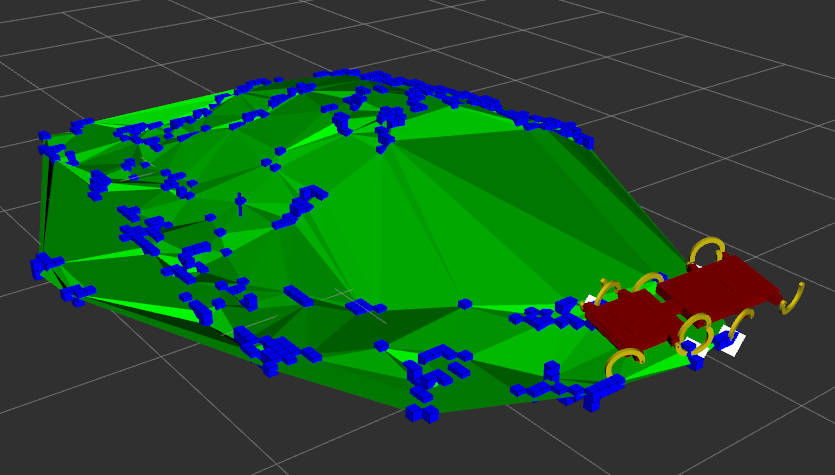
\includegraphics[height=2cm,width=1\textwidth,keepaspectratio]{../images/slides/result_research.png}
                    \caption{Следовая дорожка и полигональная сетка}
                \end{subfigure}
            \end{figure}
        \end{column}
        \begin{column}{0.49\textwidth}
            \textbf{Физико-механические свойства:}\\
            \textit{Входные данные}: обученный классификатор поверхностей, данные с внутренних датчиков робота.

            \textit{Выходные данные}: процентное соотношение упругих, твердых и пластичных свойств пройденной поверхности.

            \textit{Допустимая ошибка}: 20% 

            \vspace{-0.35cm}
            \begin{figure}[H]
                \begin{subfigure}{0.49\textwidth}
                    \centering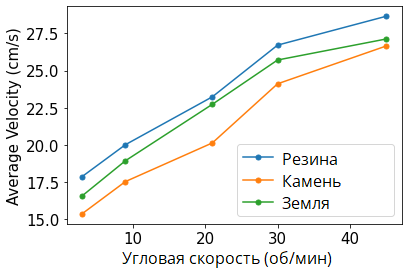
\includegraphics[height=2cm,width=1\textwidth,keepaspectratio]{../images/slides/avg_lin_vel_rev_min.png}
                    \caption*{Пример данных для обучения}
                \end{subfigure}
                \begin{subfigure}{0.49\textwidth}
                    \centering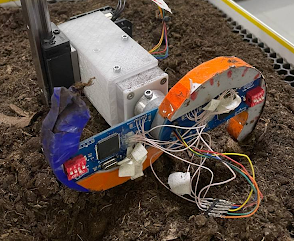
\includegraphics[height=2cm,width=1\textwidth,keepaspectratio]{../images/slides/data.png}
                    \caption*{Пример поверхности}
                \end{subfigure}
            \end{figure}
        \end{column}
    \end{columns}
\end{frame}


\begin{frame}[t]{Объект исследования}
    \framesubtitle{}
    \begin{columns}[T,onlytextwidth]
        \begin{column}{0.54\textwidth}
            \textbf{Класс многоногих шагающих роботов} с цельным или сочленённым корпусом, и цикловыми движителями с одной степенью свободы, управляемые зависимо или независимо друг от друга.

            \textit{Требования к данному классу}:
            \begin{itemize}
                \item Компактные размеры (меньше чем $1000\times600\times600$ мм)
                \item Залезать на препятствия высотой меньше, чем $\frac{3}{4}$ длины корпуса
                \item Преодолевать представленные
                      опорные поверхности
            \end{itemize}
        \end{column}
        \begin{column}{0.44\textwidth}
            \begin{figure}[H]
                \hfill
                \begin{subfigure}{0.99\textwidth}
                    \centering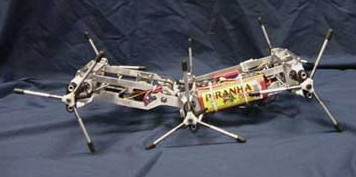
\includegraphics[height=2cm,width=1\textwidth,keepaspectratio]{from_master/whegs2.jpg}
                    \caption{WHegs}
                \end{subfigure}

                \hfill
                \begin{subfigure}{0.49\textwidth}
                    \centering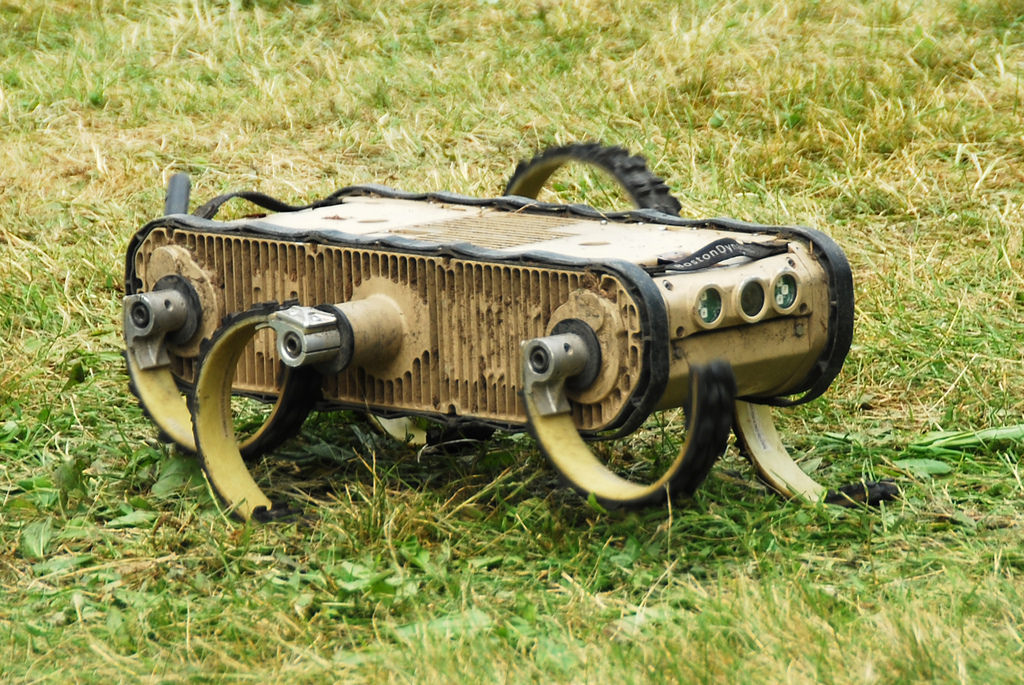
\includegraphics[height=2cm,width=1\textwidth,keepaspectratio]{from_master/rhex.jpg}
                    \caption{Boston Dynamics RHex}
                \end{subfigure}
                \begin{subfigure}{0.49\textwidth}
                    \centering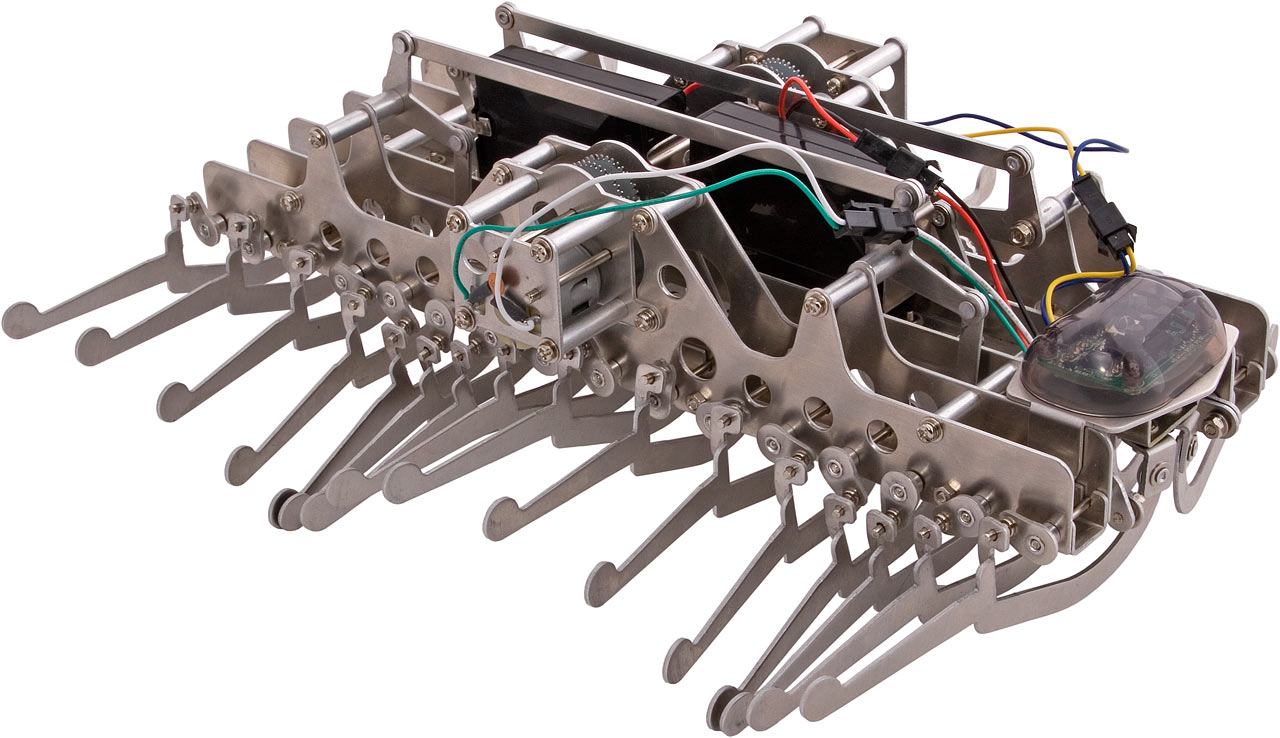
\includegraphics[height=2cm,width=1\textwidth,keepaspectratio]{from_master/gakken.jpg}
                    \caption{Gakken Centipede}
                \end{subfigure}
            \end{figure}
        \end{column}
    \end{columns}
\end{frame}

\begin{frame}[t]{"3" Оптимизация кинематической схемы}
    \framesubtitle{}
    \begin{columns}[T,onlytextwidth]
        \begin{column}{0.49\textwidth}
            Решить $F=f(x) \rightarrow max$ критерий оптимизации, где

            $f(x)$ --- критерии: пройденная дистанция, длина корпуса\\
            $(x)$ --- параметр: количество ног

            \textit{Количество ног имеет прямую зависимость с длиной корпуса робота.}
        \end{column}
        \begin{column}{0.49\textwidth}
            \vspace{-0.5cm}
            \begin{figure}[H]
                \begin{subfigure}{0.99\textwidth}
                    \centering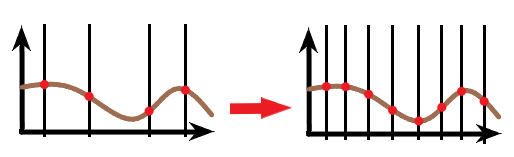
\includegraphics[height=1.8cm,width=1\textwidth,keepaspectratio]{f1.png}
                    \caption*{Кол-во ног $\uparrow$, детализация поверхности $\downarrow$}
                \end{subfigure}

                \begin{subfigure}{0.99\textwidth}
                    \centering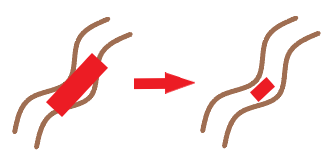
\includegraphics[height=1.8cm,width=1\textwidth,keepaspectratio]{f2.png}
                    \caption*{Длина робота $\uparrow$, курсовая проходимость $\downarrow$}
                \end{subfigure}

                \begin{subfigure}{0.99\textwidth}
                    \centering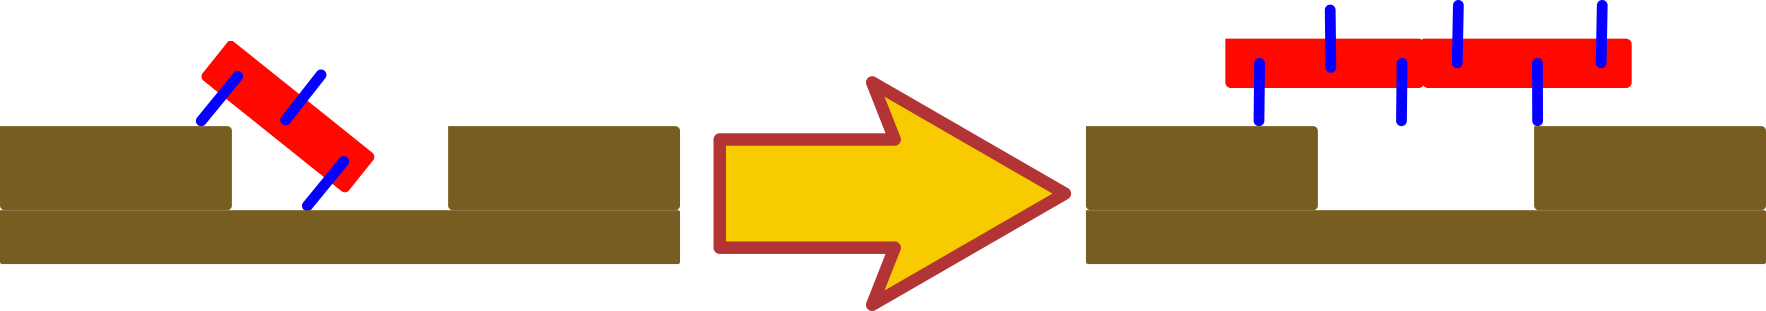
\includegraphics[height=1.8cm,width=1\textwidth,keepaspectratio]{f3_new.png}
                    \caption*{Длина робота $\uparrow$, проходимость $\uparrow$}
                \end{subfigure}
            \end{figure}
        \end{column}
    \end{columns}
\end{frame}

\begin{frame}[t]{"4" Верификация преобразователя силы}
    \framesubtitle{}
    \begin{columns}[T,onlytextwidth]
        \begin{column}{0.49\textwidth}
            Охарактеризовать материал для случаев, когда площадь приложения силы меньше, чем площадь активной части сенсора.

            \textit{Входные данные}: показания разработанного датчика и значение реально приложенной нагрузки

            \textit{Выходные данные}: разница между нормализованным значением с датчика и реальной нагрузкой

            \textit{Допустимая ошибка}: 10% 
        \end{column}
        \begin{column}{0.49\textwidth}
            \begin{figure}[H]
                \begin{subfigure}{0.9\textwidth}
                    \centering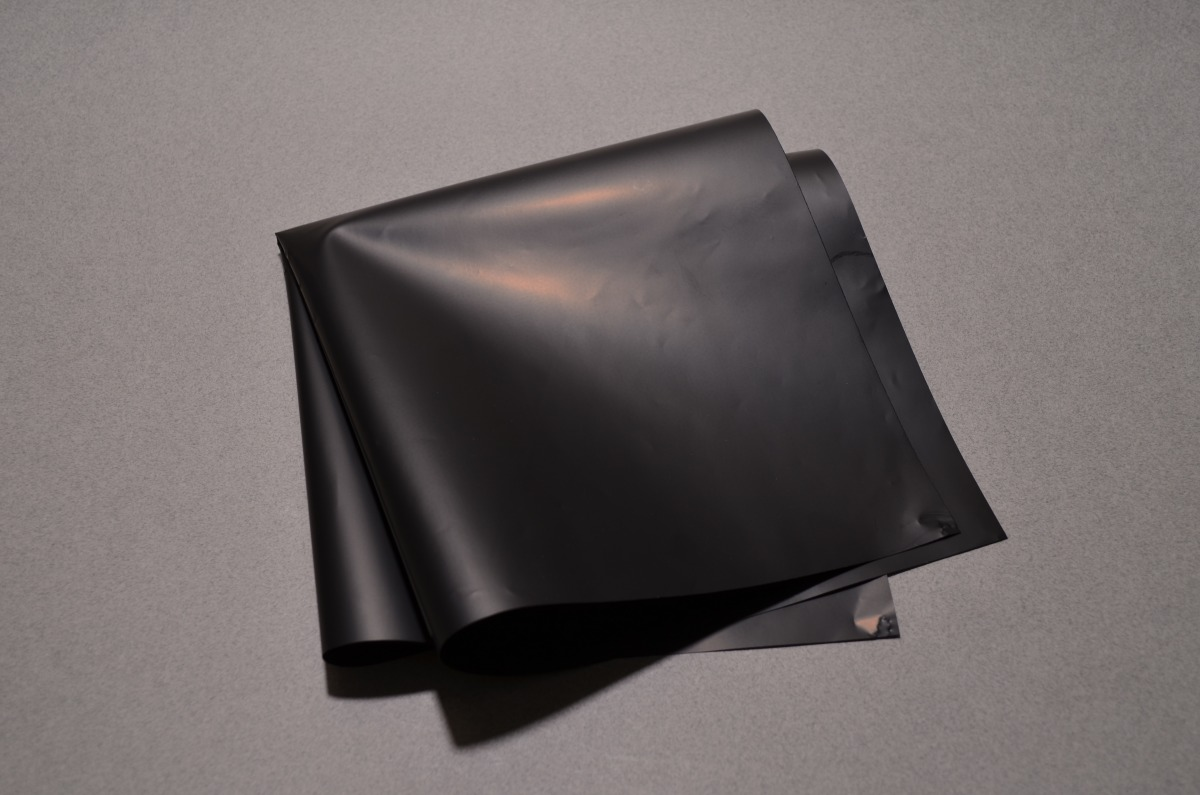
\includegraphics[height=2cm,width=1\textwidth,keepaspectratio]{velostat_sensor.jpg}
                    \caption{Материал Velostat}
                \end{subfigure}

                \begin{subfigure}{0.9\textwidth}
                    \centering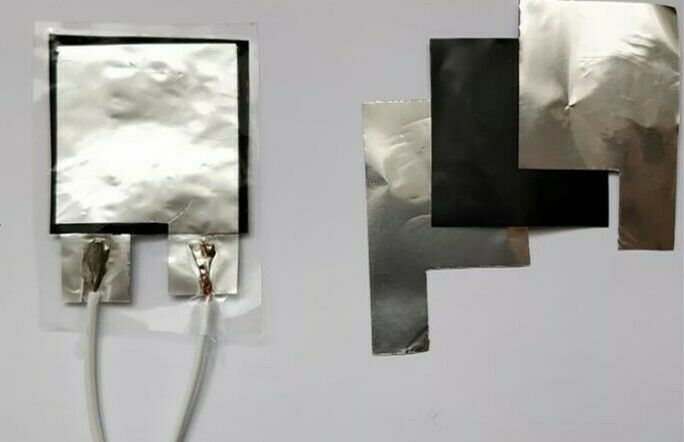
\includegraphics[height=2cm,width=1\textwidth,keepaspectratio]{simplest_sensor.jpg}
                    \caption{Простейший преобразователь силы}
                \end{subfigure}
            \end{figure}
        \end{column}
    \end{columns}
\end{frame}

\begin{frame}[t]{Структура}
    \framesubtitle{}
    \begin{figure}[H]
        \centering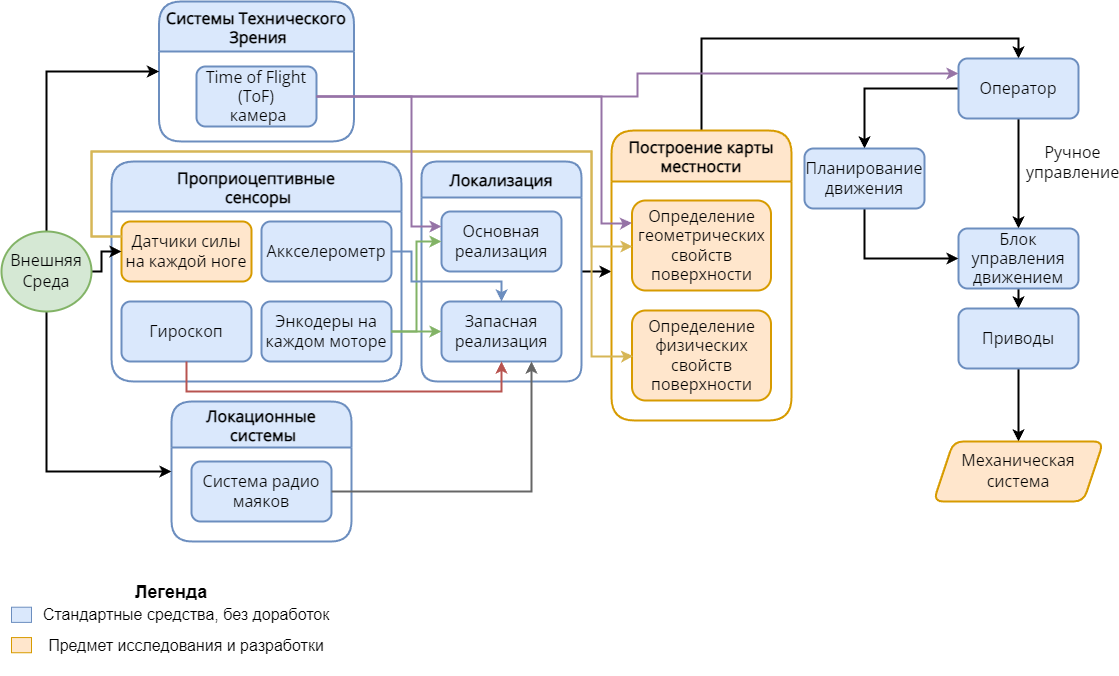
\includegraphics[height=6.5cm,width=1\textwidth,keepaspectratio]{main_diag_hor.png}
    \end{figure}
\end{frame}

\begin{frame}[t]{Основные научные задачи исследования}
    \framesubtitle{}
    \begin{enumerate}
        \item  Разработка метода \textbf{построения карты местности и определения геометрических свойств поверхности} с помощью тактильного очувствления.
        \item Реализация алгоритма, позволяющего \textbf{определять физические свойства} опорной поверхности.
        \item Разработка метода \textbf{оптимизации конструкции многоногих шагающих роботов} с цикловыми движителями с одной степенью свободы критериям проходимости, покрытия опорной поверхности и её детализации, длины пройденного пути.
        \item Создание методики \textbf{исследования датчика силы}, когда площадь контакта нажатия на сенсор меньше чувствительной области самого сенсора.
    \end{enumerate}
\end{frame}

\begin{frame}{Положения, выносимые на защиту}
    \begin{enumerate}
        \vspace{-0.3cm}
        \small
        \item \textbf{Метод построения карты местности}, состоящий в определении геометрической формы поверхности с помощью тактильного очувствления, который позволяет решать задачу определения плана и профиля поверхности в условиях отсутствия видимости и при движении по поверхности, находящейся под водой.
        \item \textbf{Метод определения физико-механических свойств опорной поверхности} на основе \textbf{тактильного очувствления}, позволяющий различать материалы с \textit{упругими, жёсткими, пластичными свойствами}.
        \item \textbf{Критерий оптимизации} кинематической схемы многоногих шагающих роботов с цикловыми одностепенными движителями, включающий в себя показатели проходимости, покрытия опорной поверхности и её детализации. Определение на его основе габаритов и количества движителей шагающего робота.
        \item \textbf{Зависимость} \textit{погрешности} датчика силы на основе полимерного материла от \textit{площади пятна контакта} относительно размеров датчика, применяемого для тактильного очувствления мобильного робота. \textbf{Методика} роботизированного исследования датчика силы.
    \end{enumerate}
\end{frame}

\section{Обзор существующих решений}

\begin{frame}[t]{Литературный обзор}
    \framesubtitle{}
    \begin{itemize}
        \item \textbf{Задача оптимизации конструкции}: Б. Петриашвили (СССР), Stefano Nolfi (Италия), Dario Sanch-Pradel (Италия), S. Feng (США)
        \item \textbf{Шагающие цикловые роботы}: Е. С. Брискин (Россия), Ю. Д. Андриантов (СССР), Edward Z. Moore (Канада), Wei-Hsi Chen (Китай)
        \item \textbf{Верификация Velostat}:  Igor Vehec (Словакия),  Robert Schroer (США)
        \item \textbf{Определение геометрических свойств поверхности}: Tobias Ebert (Германия), Subodh Kumar (США), И. Рядчиков (Россия), Shan Luo (Британия)
        \item \textbf{Определение физико-механических свойств поверхности}: X. Alice Wu (США), Krzysztof Walas (Польша), Hendrik Kolvenbach (Швейцария)
    \end{itemize}
\end{frame}